\documentclass[hyperref={colorlinks,citecolor=blue,linkcolor=blue,urlcolor=blue}]{beamer}

% For more themes, color themes and font themes, see:
% http://deic.uab.es/~iblanes/beamer_gallery/index_by_theme.html
%
\mode<presentation>
{
  \usetheme{Madrid}       % or try default, Darmstadt, Warsaw, ...
  % \usecolortheme{default} % or try albatross, beaver, crane, ...
  \usefonttheme{default}    % or try default, structurebold, ...
  \setbeamertemplate{navigation symbols}{}
  \setbeamertemplate{caption}[numbered]
} 

\usepackage[english]{babel}
\usepackage[utf8x]{inputenc}
\usepackage{chemfig}
\usepackage[version=3]{mhchem}

% On Overleaf, these lines give you sharper preview images.
% You might want to `comment them out before you export, though.
% \usepackage{pgfpages}
% \pgfpagesuselayout{resize to}[%
%   physical paper width=8in, physical paper height=6in]

% Here's where the presentation starts, with the info for the title slide
\title[]{HOW ACQUISITIONS AFFECT FIRM BEHAVIOR AND PERFORMANCE: EVIDENCE FROM THE DIALYSIS INDUSTRY \\ 
PAUL J. ELIASON et. al, 2023}
\author{Presented by: Han Zhang}
\institute{UT Austin}
\date{}

\begin{document}

\begin{frame}
  \titlepage
\end{frame}

\begin{frame}{Outline}
  \tableofcontents
\end{frame}

\section{Background}
\subsection{Introduction}
\begin{frame}{Introduction}
\begin{itemize}
    \item Research Question:
    
    How do mergers and acquisitions in the healthcare industry, particularly in outpatient dialysis facilities, impact treatment strategies, patient outcomes, and healthcare expenditures?
    \item Motivation:
    \begin{itemize}
        \item  Healthcare markets are increasingly concentrated due to M\&A
    \item While previous studies have explored associations between market structure and outcomes, there's a lack of understanding regarding the specific mechanisms driving changes in outcomes post-acquisition.
    \item This research aims to fill this gap by examining large chains implement their strategies in acquired facilities and leverage economies of scale to influence care quality and costs.
    \end{itemize}
    
\end{itemize}

\end{frame}
\begin{frame}{Literature}

\begin{itemize}
    \item Contribution to Mergers and Acquisitions Literature:
    \begin{itemize}
    \item Adds to the understanding of mergers and acquisitions effects, particularly in healthcare.
    \item Contrasts with existing literature by focusing not only on price effects but also on quality outcomes post-acquisition.
   \end{itemize}

    \item Contribution to "Roll-up" Strategies Literature

    \item Contribution to Dialysis Industry Economics Literature (e.g., Dai 2014; Dai and Tang 2015; Wilson 2016a, 2016b; Cutler, Dafny, and Ody 2017; Grieco and McDevitt 2017; Gaynor, Mehta, and Richards-Shubik 2018; Eliason 2019)
\end{itemize}

\end{frame}
\subsection{The Dialysis Industry}
\begin{frame}{Medical Background}
    
End-Stage Renal Disease (ESRD):
    \begin{itemize}
        \item Diagnosed when kidneys fail to perform these functions adequately.
        \item Survival options: kidney transplant or dialysis.
    \end{itemize}
    
Dialysis:
    \begin{itemize}
        \item Hemodialysis or peritoneal dialysis.
        \item Over 90\% of patients choose in-center hemodialysis.
    \end{itemize}

Anemia Treatment:
    \begin{itemize}
        \item Most ESRD patients receive treatment due to erythropoietin deficiency, using EPO and intravenous iron analogs, such as Venofer or Ferrlecit.
    \end{itemize}

\end{frame}
\begin{frame}{Medical Background}
A dialysis facility’s quality of care may be assessed through \textbf{clinical indicators} and \textbf{patient outcomes}.

Clinical Indicators for Dialysis Facility Quality:
\begin{itemize}
    \item Urea Reduction Ratio (URR): Measures waste filtration during dialysis.
    \item Hemoglobin (Hgb) Levels: Indicates anemia severity.
\end{itemize}

Patient Outcomes:
\begin{itemize}
    \item Mortality and hospitalization rates.
    \item especially septicemia (which can be reduced by properly cleaning machines) and cardiovascular (events exacerbated by excessive EPO use)
\end{itemize}
\end{frame}
\begin{frame}{the Role of Medicare in Dialysis}
Medicare Coverage for ESRD Patients:
\begin{itemize}
    \item After 90 days of ESRD diagnosis, all patients become eligible for Medicare coverage, regardless of age.
    \item Over 80\% of ESRD patients receiving dialysis in the US are enrolled in Medicare.
\end{itemize}

Medicare Reimbursement Policy:
\begin{itemize}
    \item Medicare pays a composite rate of around \$128 per dialysis treatment, up to three times a week per patient.
    \item Injectable drugs are reimbursed separately based on the quantity administered.
\end{itemize}



\end{frame}
\begin{frame}{the Market for Dialysis}
Market dominated by for-profit chains like DaVita and Fresenius, controlling over 60\% of facilities and earning 90\% of revenue.

Advantages of Dialysis Chains:
\begin{itemize}
    \item Potential lower costs due to volume discounts and centralized services.
    \item Stronger bargaining position with commercial insurance companies.
\end{itemize}

Standardization and Operation Manuals:
\begin{itemize}
    \item Chains implement firm-wide standards and operation manuals.
\end{itemize}

Quality Concerns:
\begin{itemize}
    \item filthy or unsafe conditions, excessive use of injectable drugs, and potential discouragement of kidney transplants.
    \item Lawsuits against providers and scrutiny by regulatory bodies.
\end{itemize}

\end{frame}


\section{Data}
\begin{frame}{Data}

Patient- and facility-level data from the United States Renal Data System (USRDS).
Patient Data:
\begin{itemize}
    \item  includes demographic information, cause of ESRD, comorbidities, residential ZIP Code, facility of treatment, mortality data, transplant status, and waitlist status.
\end{itemize}
Facility Data:
\begin{itemize}
    \item Includes facility ID, address, chain affiliation, labor inputs, number of dialysis stations, for-profit status, and types of treatment offered.
\end{itemize}

Acquisition Data:
\begin{itemize}
    \item Precise acquisition dates obtained from Provider of Service files and annual cost reports submitted to CMS.
\end{itemize}

\end{frame}
\begin{frame}{Descriptive Statistics}
    \begin{figure}
        \centering
        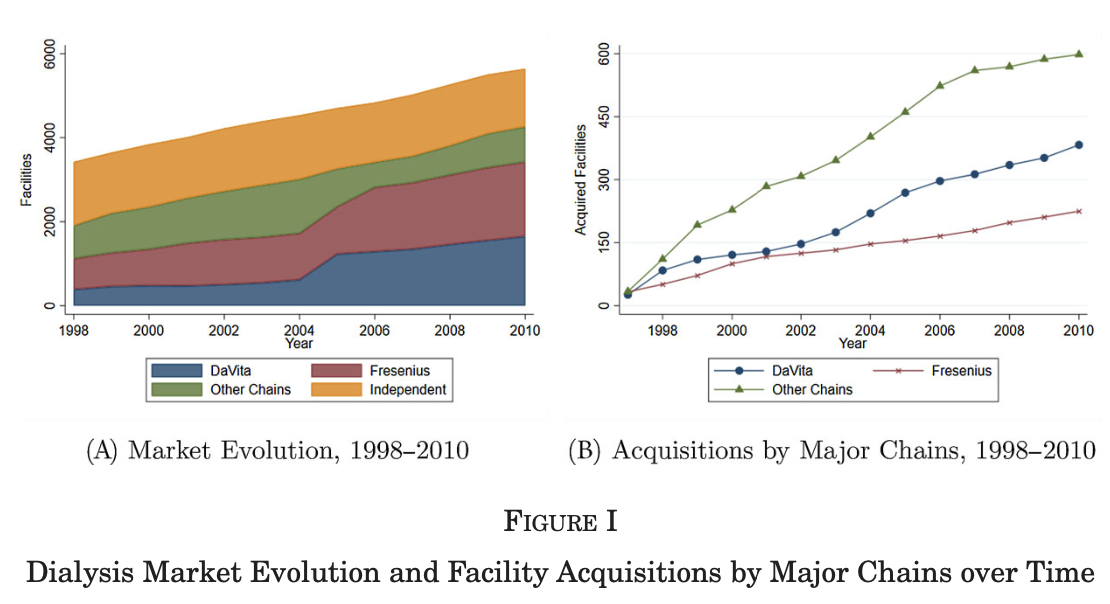
\includegraphics[width=0.9\linewidth]{fig1.png}
    \end{figure}
\end{frame}
\begin{frame}{Descriptive Statistics}
    \begin{figure}
        \centering
        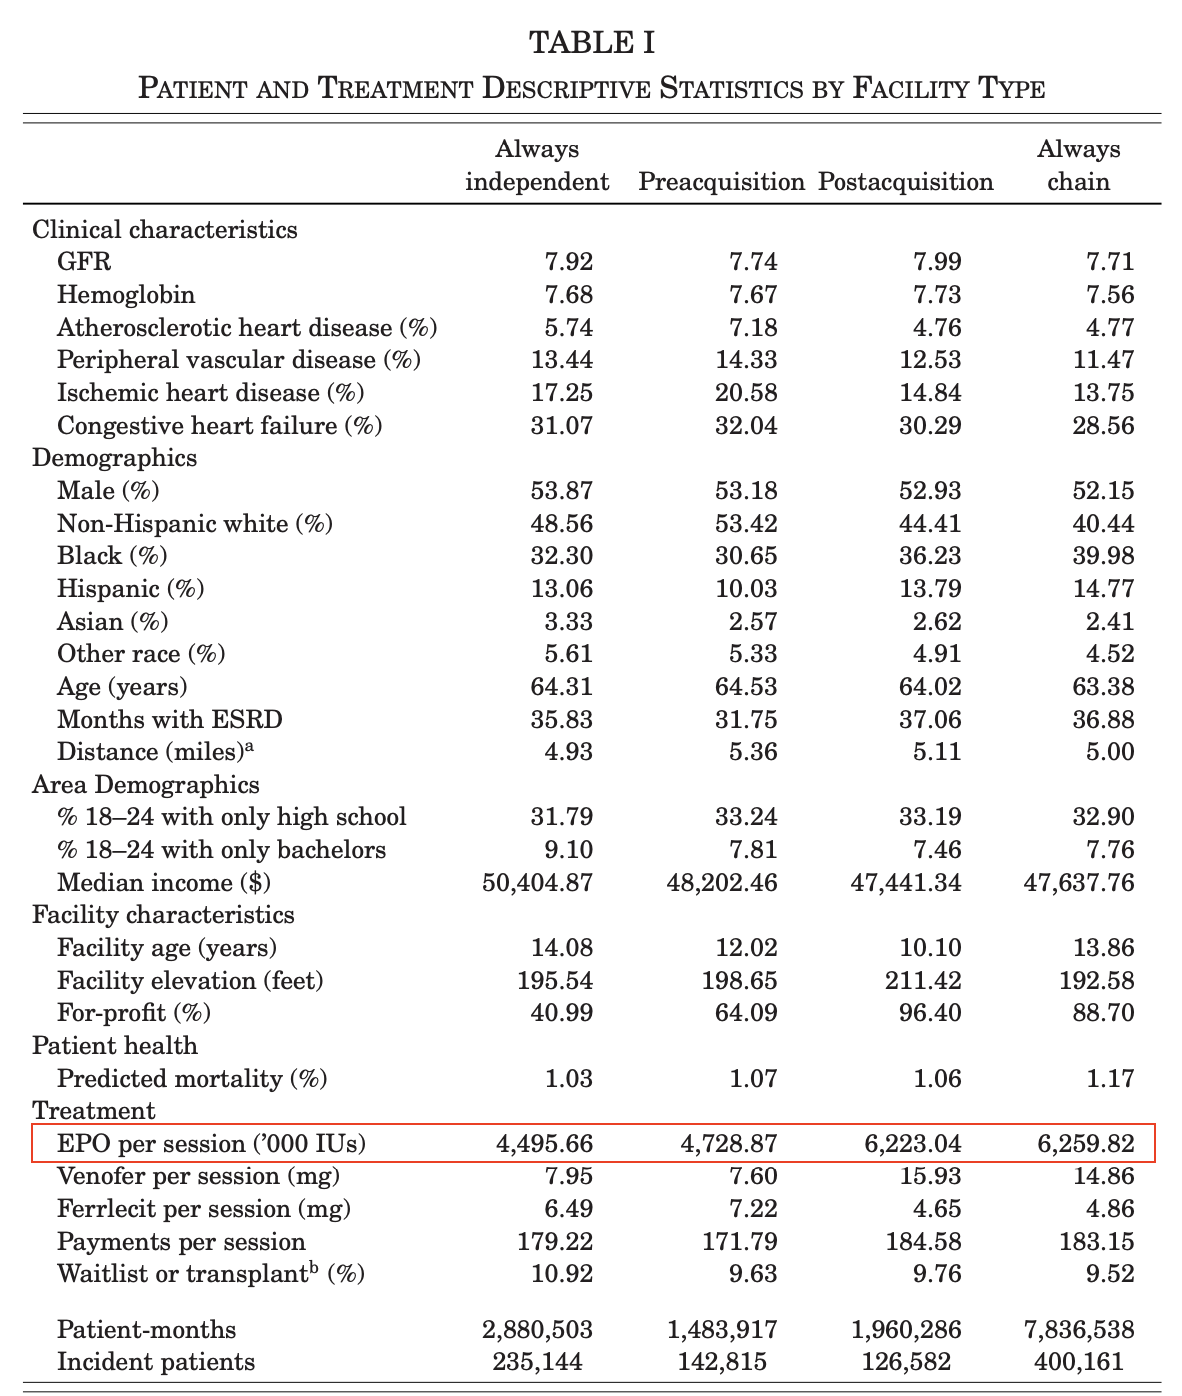
\includegraphics[width=0.5\linewidth]{tb1.png}
    \end{figure}
    
\end{frame}
\begin{frame}{Descriptive Statistics}
No systematic differences across facility types for many attributes.

    Treatment Disparities:
    \begin{itemize}
        \item Patients at chain-owned facilities receive more EPO per session and are more likely to receive Venofer than Ferrlecit.
        \item  Payments per session increase by about 7\% at facilities acquired by a chain.
    \end{itemize}
    
       
\end{frame}
\begin{frame}{Descriptive Statistics}
    \begin{figure}
        \centering
        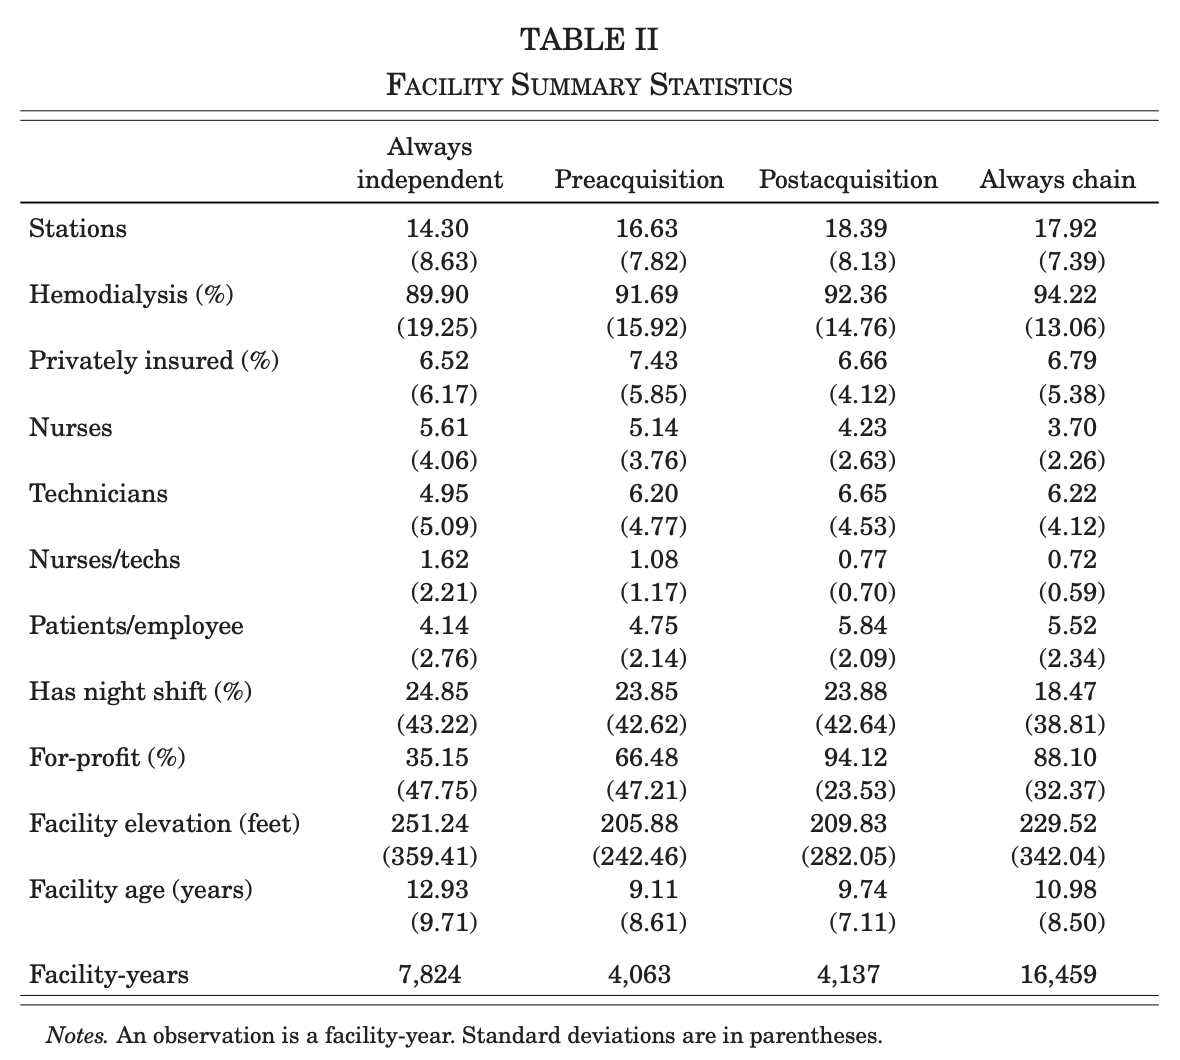
\includegraphics[width=0.5\linewidth]{tb2.png}
    \end{figure}
    chain-owned facilities:
    \begin{itemize}
        \item substitute toward lower-cost technicians and away from higher-cost nurses
        \item treating more patients per employee.
    \end{itemize}
\end{frame}

\section{the Effects of Acquisitions}
\begin{frame}{THE IMPACT OF ACQUISITIONS }
    difference-in-differences research design that compares independent facilities acquired by chains to those that are never acquired:
    $$Y_{ijt} = \beta_{pre}D^{Pre}_{jt} + \beta_{post}D^{post}_{jt} + \beta_{chain}D^{chain}_{jt} + \alpha X_{ijt} + \epsilon_{ijt} $$

\begin{itemize}
    \item $Y_{ijt}$ is the outcome of interest for patient $i$ at facility $j$ in month $t$;
    \item $D_{pre}$ and $D_{Post}$ are indicators for whether facility $j$ in
month $t$ will be acquired in the future or has already been acquired;
    \item $D_{Chain}$ is an indicator for whether facility j is always owned by a chain.
\end{itemize}

To avoid measurement error in the date of acquisition and to allow enough time for a firm’s strategy to be fully implemented, exclude all observations within a six-month window on either side of the acquisition date.

\end{frame}
\begin{frame}{Identification Threats and Remedies}
Primary Threat to Identification:
\begin{itemize}
    \item Chains may acquire independent facilities with patients having characteristics affecting outcomes through channels unrelated to ownership change.
\end{itemize}

Overcoming Identification Challenges:
\begin{itemize}
    \item Patients treated at acquired independent facilities are not systematically different along observable characteristics.
    \item Richness of data allows control for clinically relevant covariates
\end{itemize}
\end{frame}
\begin{frame}{the Effect of Drug Doses}
    \begin{figure}
        \centering
        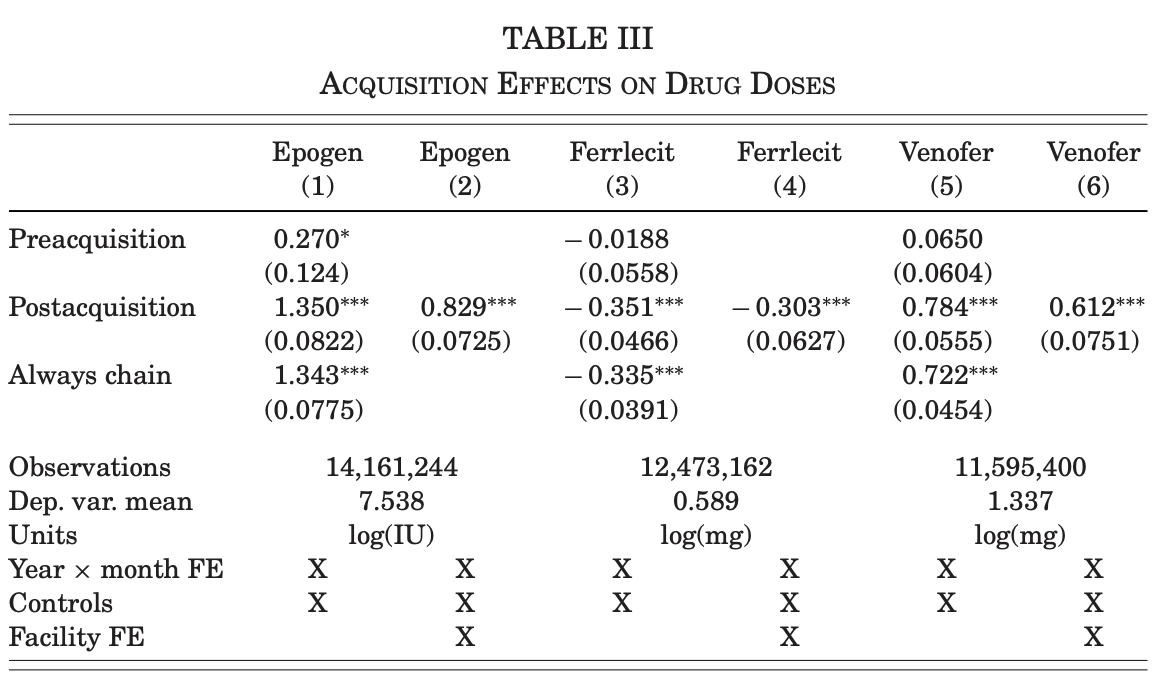
\includegraphics[width=0.7\linewidth]{tb3.png}
    \end{figure}
    \begin{itemize}
        \item substantial increase in EPO usage
        \item switch from Ferrlecit to Venofer for more profit
    \end{itemize}
\end{frame}
\begin{frame}{the Effect of Drug Doses}
    \begin{figure}
        \centering
        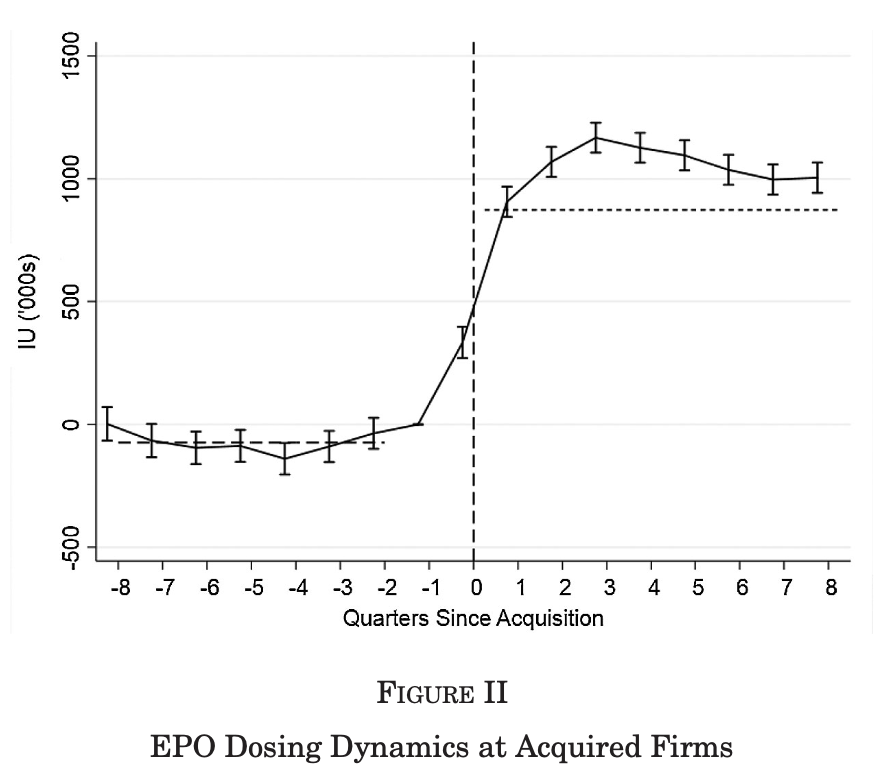
\includegraphics[width=0.5\linewidth]{fig2.png}
    \end{figure}
    $$Y_{ijt}=\sum_s \delta^sD^s_{jt} +\alpha X_{ijt} +\epsilon_{ijt}$$
    where $D_{jt}^s$ is a dummy for facility $j$ being acquired at time $t+s$
\end{frame}
\begin{frame}{the Effect on Facility Input}
    facility-year level: 
    $Y_{ijt}= \gamma^{Post}D^{Post}_{jt}+\delta X_{jt} + \nu_{jt}$
    \begin{figure}
        \centering
        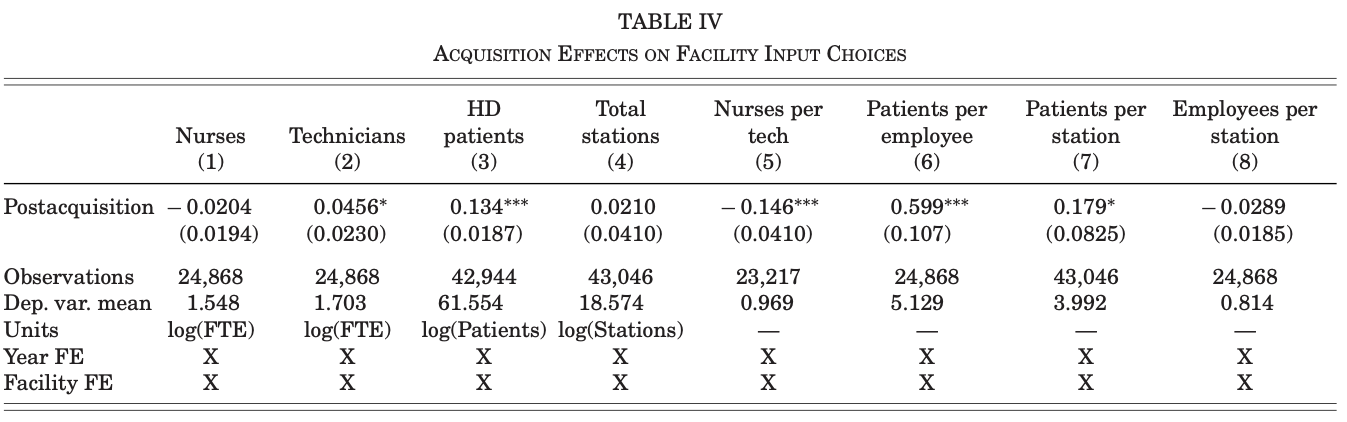
\includegraphics[width=0.8\linewidth]{tb4.png}
    \end{figure}
    upon acquisition, to reduce cost:
    \begin{itemize}
        \item switch from nurses to technicians
        \item higher patients per employee, patients per station
    \end{itemize}
\end{frame}
\begin{frame}{the Effect on Patient Outcome}
    \begin{figure}
        \centering
        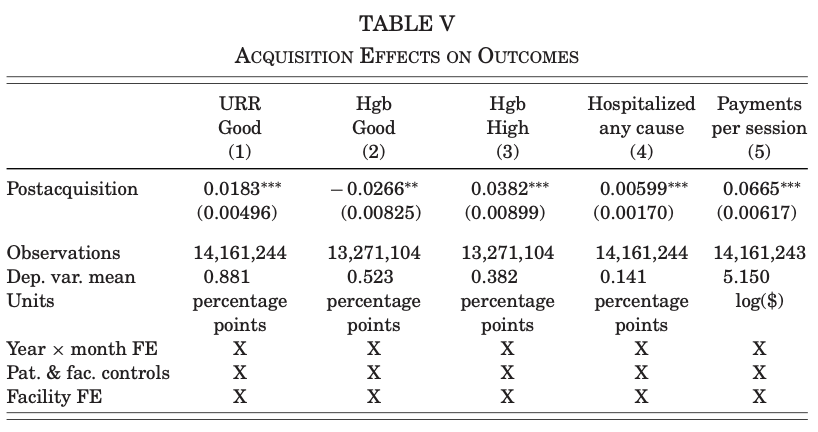
\includegraphics[width=0.8\linewidth]{tb5.png}
    \end{figure}
    \begin{itemize}
        \item Higher Hgb due to larger EPO usage
        \item increased hospitalization, especially for septicemia and cardiac events
        \item increased Medicare expenditure
    \end{itemize}
\end{frame}
\begin{frame}{the Effect on Patient Outcome}
    \begin{figure}
        \centering
        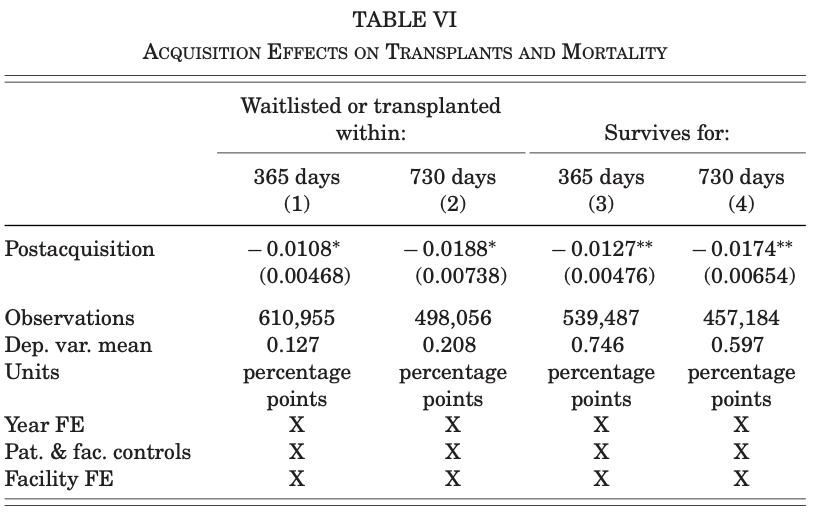
\includegraphics[width=0.8\linewidth]{tb6.png}
    \end{figure}
\end{frame}
\begin{frame}{the Effect on Patient Selection}
    \begin{figure}
        \centering
        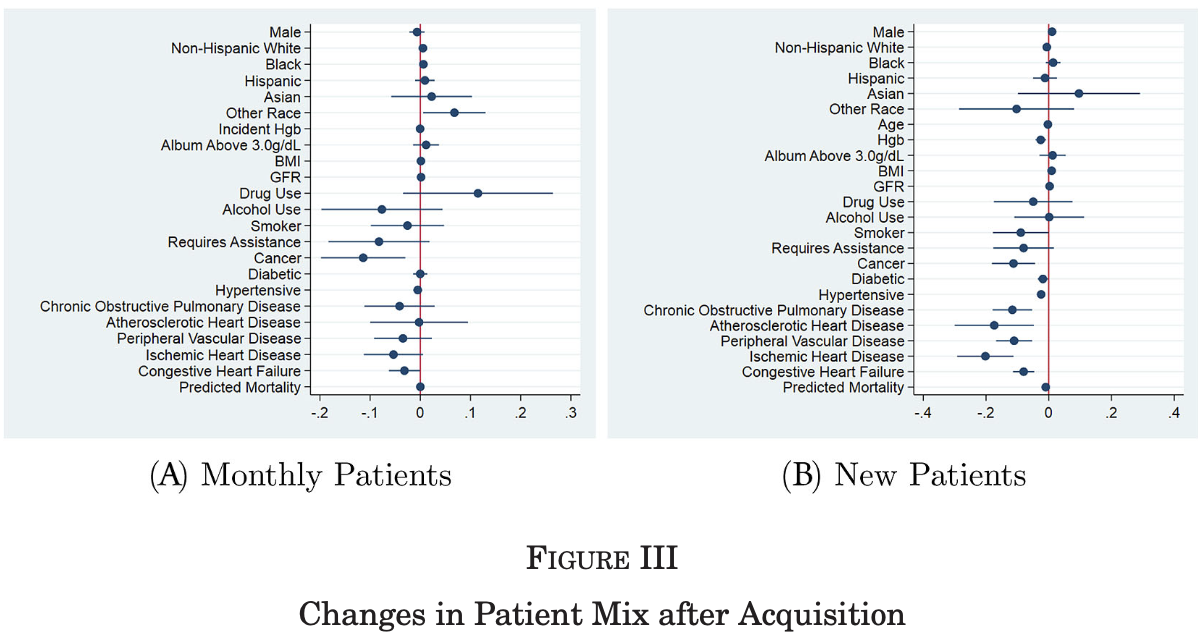
\includegraphics[width=0.8\linewidth]{fig3.png}
    \end{figure}
    $$X_{ijt} = \beta^{Post}D^{Post}_{jt}+\gamma_j+\delta_t+\epsilon_{ijt} $$
    facilities treating healthier patients: new patients at acquired facilities are less likely to have a variety of comorbid conditions

\end{frame}

\section{the Effect of Competition}
\begin{frame}{THE EFFECT OF COMPETITION ON FIRM BEHAVIOR}
    \begin{itemize}
        \item investigate whether competition from other dialysis firms can discipline the behavior of newly acquired facilities
        \item defines markets as HSAs (hospital service areas)
        \item uses a Herfindahl-Hirschman Index (HHI) to measure concentration
        \item define \textit{post-acquisition HHI} as what the HSA’s HHI would have been in the month before acquisition had the facility already been acquired, to avoid confounding the effect of acquisition with the entry of new dialysis facilities.
    \end{itemize}
\end{frame}
\begin{frame}{Change on Market Concentration}
    \begin{figure}
        \centering
        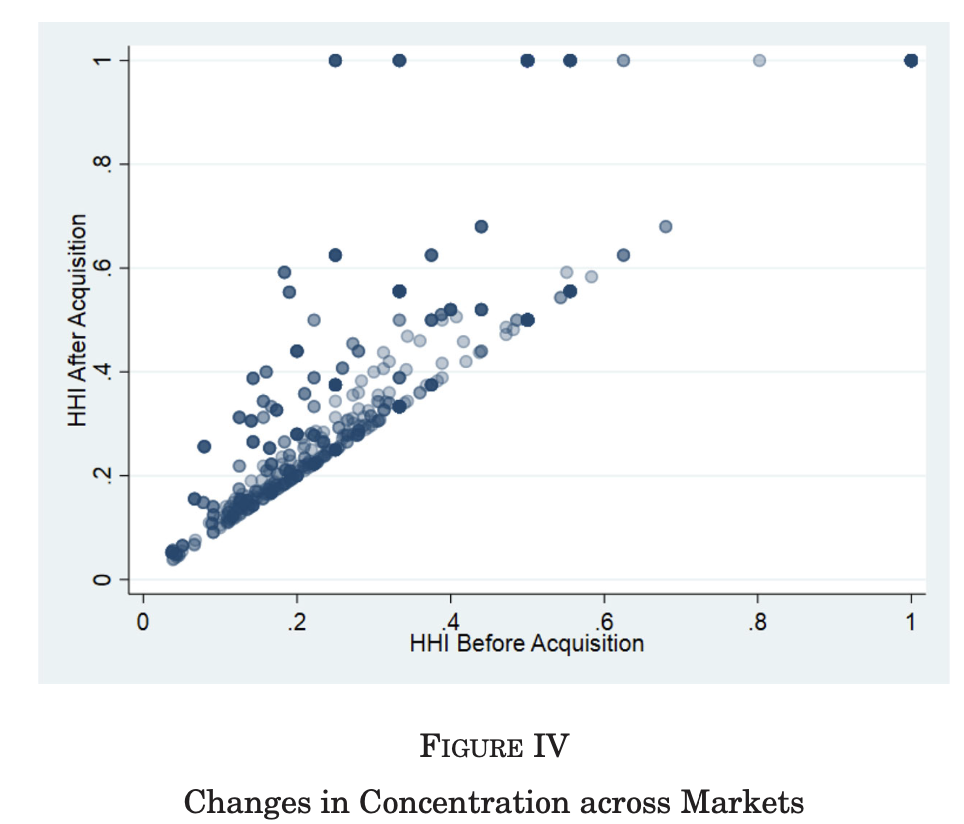
\includegraphics[width=0.6\linewidth]{fig4.png}
    \end{figure}
    \begin{itemize}
        \item HHI increases in only 34.4\% of HSA-months following an acquisition
        \item changes in facility behavior and patient outcomes are not driven by changes in market concentration
    \end{itemize}
\end{frame}
\begin{frame}{Acquisitions That Increase HHI Have Similar Effects}
    \begin{figure}
        \centering
        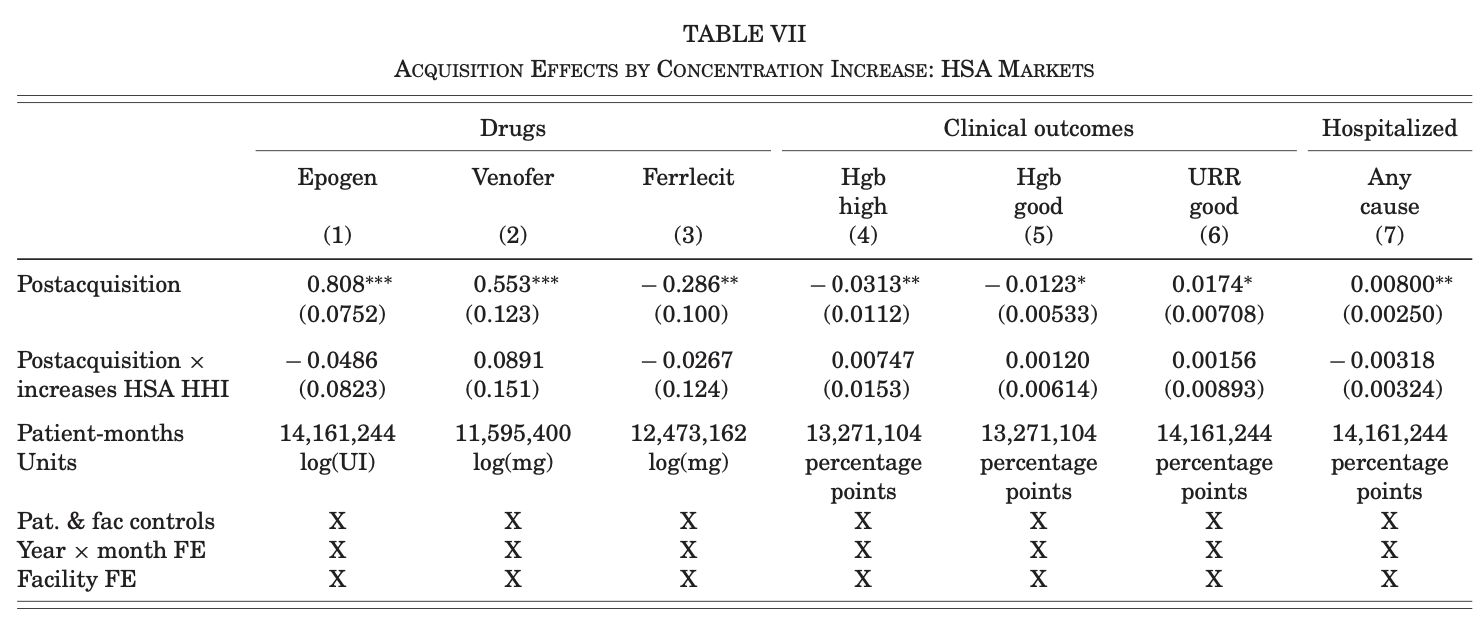
\includegraphics[width=0.8\linewidth]{tb7.png}
    \end{figure}
     $$Y_{ijt} = \beta_{Post}D^{Post}_{jt} + \gamma_{Post}D^{Post}_{jt}\times IncreasesHHI_{j} + \alpha X_{ijt} + \epsilon_{ijt} $$
% $IncreasesHHI_j$ : dummy if the acquisition of facility $j$ increased HHI. 
    \begin{itemize}
        \item the outcomes in markets where an acquisition increased concentration do not differ from those where an acquisition did not
        \item therefore, the decrease in quality of care occurs through the transference of firm strategy, not an increase in market power.
    \end{itemize}

\end{frame}
\begin{frame}{Why Competition Does Not Discipline Provider Behavior}
    \begin{figure}
        \centering
        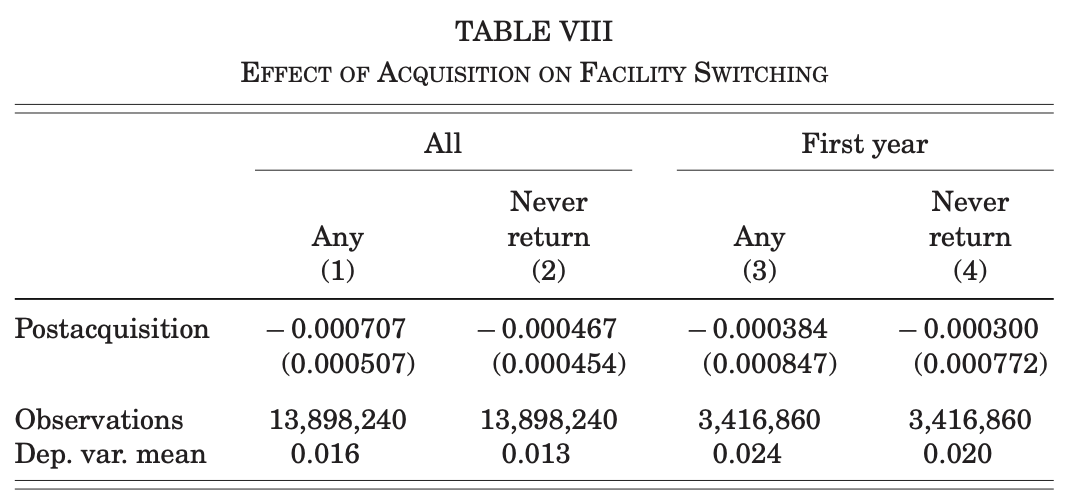
\includegraphics[width=0.7\linewidth]{tb8.png}
    \end{figure}
    \begin{itemize}
        \item standard models of competition with endogenous provider quality predict that quality will increase with competition, assuming that demand increases with product quality
        \item In practice, patient demand in the U.S. dialysis market does not respond to the decline in quality following an acquisition
        \item may be due to a lack of options and travel cost
    \end{itemize}
\end{frame}

\section{Differences Across Chains and Independent Facilities}
\begin{frame}{PREACQUISITION DIFFERENCES ACROSS CHAIN AND INDEPENDENT FACILITIES}
why independent facilities do not imitate the behavior of the more profitable chain facilities before acquisition?

estimate the impact of an acquisition on total variable profits per dialysis session and several variables related to EPO
    $$Y_{jt} = \beta_{pre}D^{Pre}_{jt} + \beta_{post}D^{post}_{jt} + \beta_{chain}D^{chain}_{jt} + \alpha X_{jt} + \epsilon_{jt} $$
\end{frame}
\begin{frame}{PREACQUISITION DIFFERENCES ACROSS CHAIN AND INDEPENDENT FACILITIES}
\begin{figure}
    \centering
    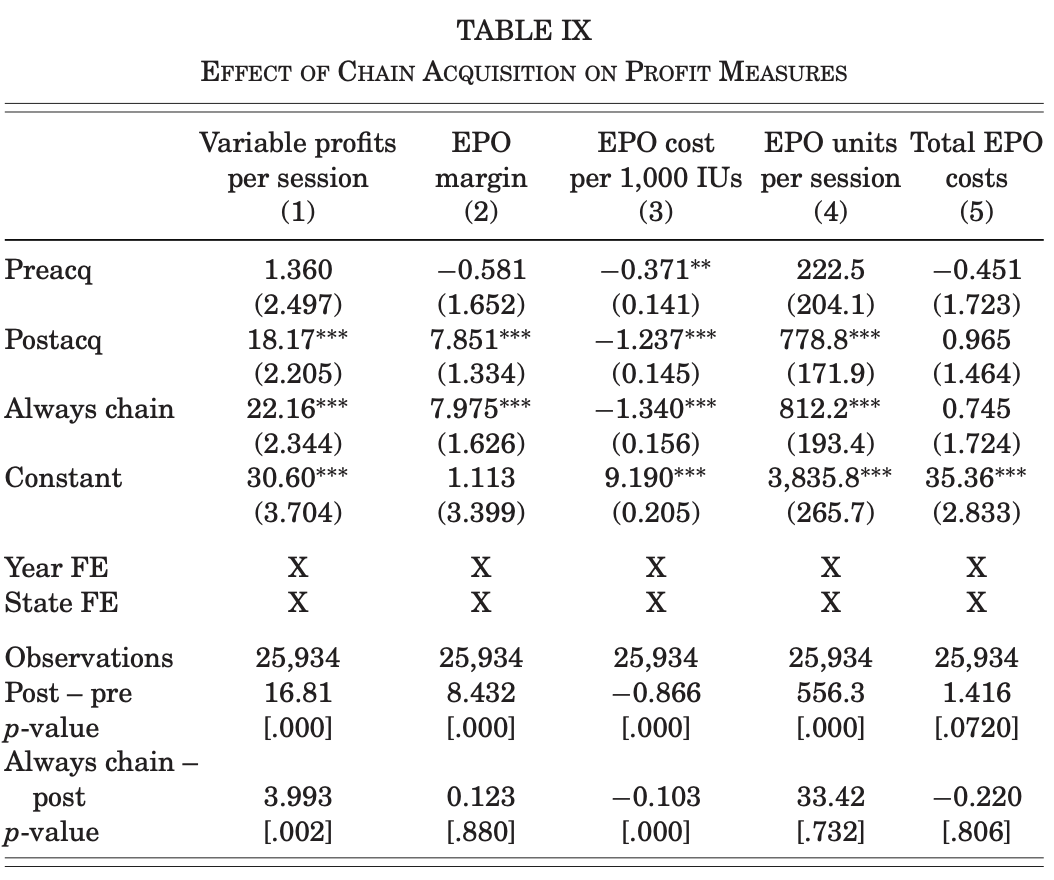
\includegraphics[width=0.6\linewidth]{tb9.png}
\end{figure}
\end{frame}
\begin{frame}{PREACQUISITION DIFFERENCES ACROSS CHAIN AND INDEPENDENT FACILITIES}

Profit Composition at Acquired Facilities:
\begin{itemize}
    \item Majority of per-session profit increase at acquired facilities attributed to EPO.
    \item Chains pay lower prices for EPO due to negotiated volume discounts with drug suppliers-- scale economies from buyer power not available to smaller independent facilities.
\end{itemize}

Objectives and Incentives:
\begin{itemize}
    \item Chains may prioritize financial performance over patient outcomes.
\end{itemize}

Risks and Financial Reserves:
\begin{itemize}
    \item Chains may accept risks on patient care due to financial reserves to cover litigation costs, highlighted by instances of large settlements by chains like DaVita.
\end{itemize}

\end{frame}

\section{Conclusion}
\begin{frame}{Conclusion}

Changes in Behavior at Acquired Facilities:
    \begin{itemize}
        \item Increase per-session reimbursements from Medicare by elevating drug doses and shifting to more lucrative drugs.
        \item Optimize resource utilization by treating more patients with the same staff and stations.
        \item Cut costs by replacing high-skill nurses with lower-skill technicians.
    \end{itemize}

Effect on Patient Outcomes:
  \begin{itemize}
      \item Quality of care declines at acquired facilities
      \item Medicare spending increases
  \end{itemize}



\end{frame}
\begin{frame}{Conclusion}
Policy Implications:
  \begin{itemize}
      \item Current antitrust laws may not address the harmful effects of acquisitions that impact care quality rather than market concentration.
      \item Policies like certificate of need laws and reimbursement structures could inadvertently drive consolidation.
  \end{itemize}

Broader Applications and Future Research:
  \begin{itemize}
      \item Lessons from dialysis industry acquisitions applicable to other healthcare and education sectors.
  \end{itemize}
\end{frame}

\end{document}